% Generator: hand-authored TikZ schematic; coordinates are not to scale.
% Source: fixed 2006 Liaoning arts candidate PDF, source ID
% src-b784613ebc50375b17eb4a91083b447879ebb9ed75bb6a76227bb74345cfbfd3,
% SHA-256 bbb83af465d4650c594f23a879d82dea43a86f805b6fc8712d25809aac7fda22,
% PDF page 1, printed page 310, Q15.
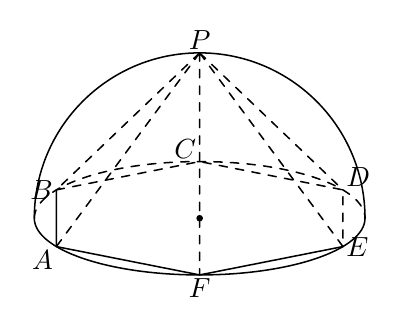
\begin{tikzpicture}[line cap=round,line join=round,line width=0.55pt]
  % Schematic perspective of the hemisphere and the inscribed regular hexagon.
  \coordinate (P) at (0,2.70);
  \coordinate (A) at (-1.82,0.24);
  \coordinate (B) at (-1.82,0.96);
  \coordinate (C) at (0,1.32);
  \coordinate (D) at (1.82,0.96);
  \coordinate (E) at (1.82,0.24);
  \coordinate (F) at (0,-0.12);

  % Outer profile of the hemisphere and its equatorial rim.
  \begin{scope}[shift={(0,0.60)}]
    \draw (-2.10,0) arc (180:0:2.10);
    \draw[dashed] (-2.10,0) arc (180:0:2.10 and 0.72);
    \draw (2.10,0) arc (0:-180:2.10 and 0.72);
  \end{scope}

  % Hidden rear edges of the base hexagon and all pyramid edges inside the dome.
  \draw[dashed] (B)--(C)--(D)--(E);
  \draw[dashed] (P)--(A) (P)--(B) (P)--(C) (P)--(D) (P)--(E) (P)--(F);
  % Visible front edges of the base hexagon.
  \draw (E)--(F)--(A)--(B);

  % Unlabelled center mark shown in the source diagram.
  \fill (0,0.60) circle (1.2pt);
  \node[above,inner sep=1pt] at (P) {$P$};
  \node[below left,inner sep=1pt] at (A) {$A$};
  \node[left,inner sep=1pt] at (B) {$B$};
  \node[above left,inner sep=1pt] at (C) {$C$};
  \node[above right,inner sep=1pt] at (D) {$D$};
  \node[right,inner sep=1pt] at (E) {$E$};
  \node[below,inner sep=1pt] at (F) {$F$};
\end{tikzpicture}
